\documentclass{fmbvecto}

\usepackage[spanish]{babel}
\usepackage{caption}

\renewcommand{\title}{Taller 3}
\newcommand{\subject}{Cálculo Vectorial}

\renewcommand{\labelenumii}{\theenumii}
\renewcommand{\theenumii}{\theenumi.\arabic{enumii}.}

\NewDocumentCommand{\itemp}{o}{\item (#1 puntos)}

\begin{document}

Jueves, 18 de julio de 2024

\begin{center}
    \textbf{\LARGE \title} \\
    {\large \subject}
\end{center}


Profesor: Jacinto Eloy Puig Portal, \href{mailto:jpuig@uniandes.edu.co}{jpuig@uniandes.edu.co}. \\
Monitor: Federico Melo Barrero, \href{mailto:f.melo@uniandes.edu.co}{f.melo@uniandes.edu.co}.\\

\textbf{\Large Preámbulo}

Las instrucciones referentes a la entrega del taller están escritas en \href{https://bloqueneon.uniandes.edu.co/d2l/home}{Bloque Neón}.

\subsection*{Indicación}

Resuelva únicamente un ejercicio de cada sección. Si resuelve más de uno, se calificará alguno arbitrariamente.

\subsection*{Bonos}
\begin{itemize}
  \item Se sumarán 0.25 puntos de bonificación a la nota del taller si su contenido está ordenado y puede leerse con facilidad.
  \item Se sumarán 0.25 puntos de bonificación a la nota del taller si no contiene errores léxicos, gramaticales ni faltas de ortografía.
\end{itemize}
La nota del taller puede exceder el 5.0.

\subsection*{Recomendaciones}

No necesita hacer uso de herramientas que le ayuden a hacer matemáticas, ya sean calculadoras, aplicaciones, grandes modelos de lenguaje u otras. Le recomiendo que no lo haga.

Recuerde incluir las unidades siempre que trate con magnitudes físicas.


\section{Taller 2}

\begin{enumerate}

\item (1.25 puntos) Corrija todos los errores que tuvo en el taller 2. Si no tuvo errores, omita este punto.

\end{enumerate}

\section{Teorema de Green}

\begin{enumerate}

\item (1.25 puntos) Sea \(\bvec{F}\colon \mathbb{R}^2 \to \mathbb{R}^2\) el campo vectorial dado por
\[
  \bvec{F}(x, y) = (\mathrm{e}^{-x} + y^2, \mathrm{e}^{-y} + x^2).
\]
y sea \(D\) una región cuya frontera consiste de la unión entre:
\begin{itemize}
  \item El arco de la curva \(y = \cos x\) que abarca entre los puntos \(\left(-\frac{\uppi}{2}, 0\right)\) y \(\left(\frac{\uppi}{2}, 0\right)\).
  \item El segmento de recta que va desde \(\left(\frac{\uppi}{2}, 0\right)\) hasta \(\left(-\frac{\uppi}{2}, 0\right)\).
\end{itemize}
Calcule la integral de línea de \(\bvec{F}\) sobre \(\partial D\).

\item (1.25 puntos) Sírvase del teorema de Green para probar la fórmula de cambio de variables para integrales dobles en el caso particular en el que la función a transformar es \(1\). Ya debe estar familiarizado con ella, pero en caso contrario, la fórmula es la siguiente: 
\[
  \iint_R \: \mathrm{d}x \: \mathrm{d}y = \iint_S \: \left| \frac{\partial(x, y)}{\partial(u, v)} \right| \: \mathrm{d}u \: \mathrm{d}v.
\]
\end{enumerate}

\section{Teorema de Stokes}

\begin{enumerate}

\item (1.25 puntos) Sea \(\bvec{F}\colon \mathbb{R}^3 \to \mathbb{R}^3\) el campo vectorial dado por
\[
  \bvec{F}(x, y, z) = (xyz, xy, x^2yz).
\]
y sea \(S\) la superficie que consiste de la cara de arriba y las cuatro caras laterales de un cubo de lado \(2\) centrado en el origen, con caras paralelas a los planos coordenados y orientada hacia afuera. Calcule la integral de superficie de \(\rot \bvec{F}\) sobre \(S\).

\item (1.25 puntos) Demuestre o refute que 
\[
  \int_C (f \nabla g) \cdot \mathrm{d}\bvec{r} = \iint_S (\nabla f \times \nabla g) \cdot \mathrm{d}S,
\]
donde \(C\) es una curva cerrada simple y suave, \(S\) es una superficie cerrada simple y suave, y \(f, g\) son funciones escalares de clase \(C^2\).

\end{enumerate}

\section{Teorema de Gauss}

\begin{enumerate}

\item (1.25 puntos) Considere el campo vectorial graficado en la figura \ref{fig:vector-field}. Sírvase de la interpretación geométrica del teorema de Gauss para determinar el signo de la divergencia del campo en cada uno de los puntos resaltados.

\begin{center}
  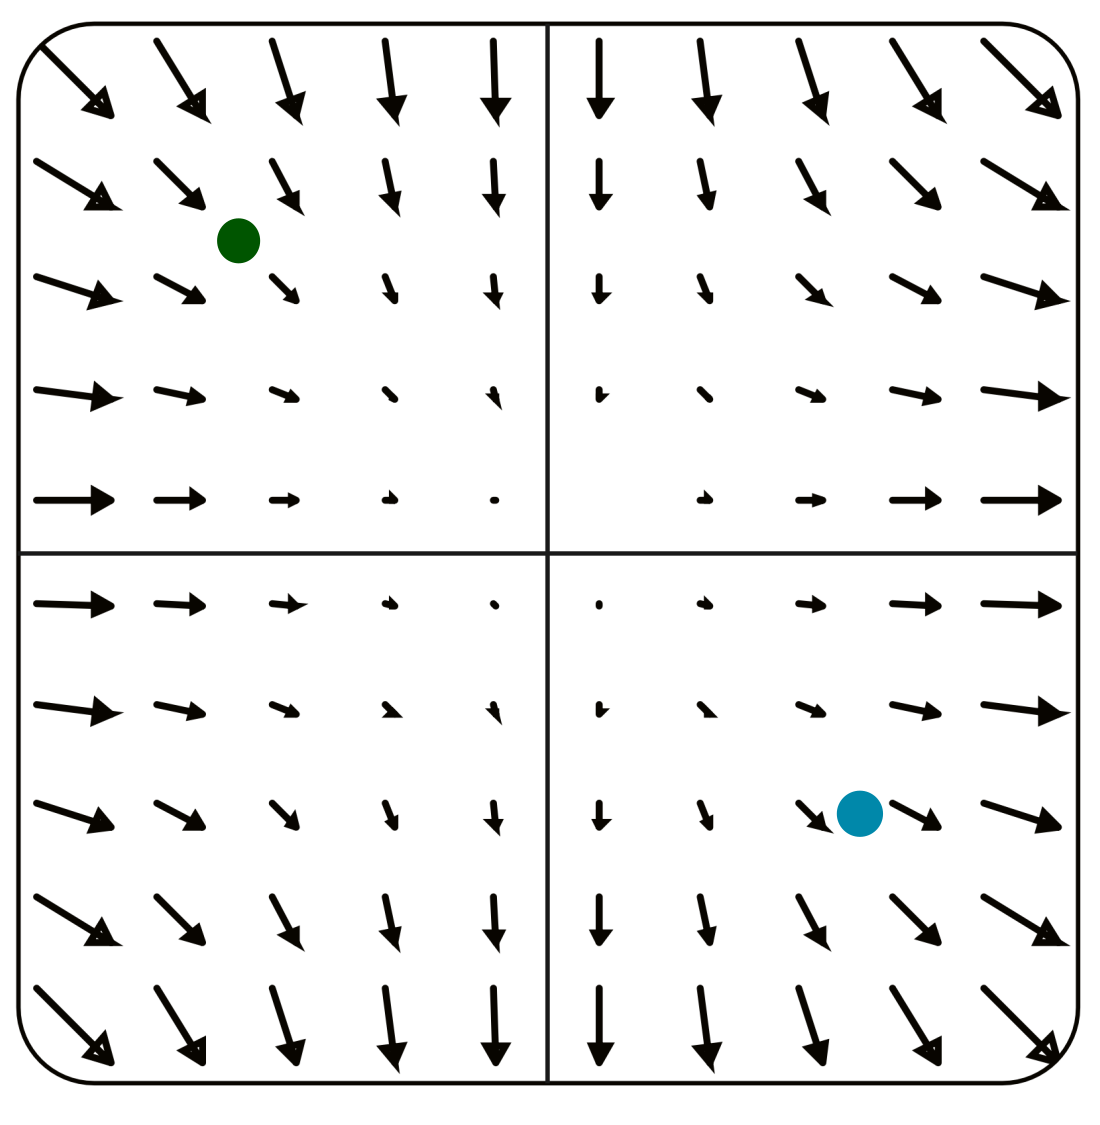
\includegraphics[width=0.4\textwidth]{vector-field.png}
  \captionof{figure}{Campo vectorial con dos puntos resaltados: uno verde y otro azul.}
  \label{fig:vector-field}
\end{center}

\vspace*{1em}

\item (1.25 puntos) Sea \(f\colon \mathbb{R}^3 \to \mathbb{R}\) el campo escalar dado por
\[
  f(x, y, z) = 2x + 2y + z^2
\]
y sea \(S\) la esfera de radio \(1\) centrada en el origen. Calcule
\[
  \iint_S f \: \mathrm{d}S.
\]

\end{enumerate}

\end{document}
